\section{Evaluation of \ac{ae}}\label{sec:evaluation-ae}

% architecture
In order to determine, which architecture for the hidden or so-called latent space of the \ac{ae} is the best option, 
different architectures were tested and compared in terms of \ac{rsme} and cosine similarity.
The \ac{rsme} is calculated as given in \lst{lst:impl-rsme}.
The cosine similarity is calculated as given in \lst{lst:impl-cos_sim}.
The dataset used for the evaluation is a selection of 195 documents from the Bahamas dataset.

% RSME
\begin{listing}[htp]
    \begin{minted}{python3}
        rsme = np.linalg.norm(inverse_embedding - embeddings) 
                / np.sqrt(embeddings.shape[0])
    \end{minted}
    \caption{
        Computation of the \ac{rsme} between the original and the reconstructed embedding.
    }
    \label{lst:impl-rsme}
\end{listing}

% cosine similarity
\begin{listing}[htp]
    \begin{minted}{python3}
        cos_sim = statistics.mean([np.dot(inverse_emb, embedding)
                /(np.linalg.norm(inverse_emb)*np.linalg.norm(embedding)) 
                for inverse_emb, embedding in zip(inverse_embedding, embeddings)])
    \end{minted}
    \caption{
        Computation of the cosine similarity between the original and the reconstructed embedding.
    }
    \label{lst:impl-cos_sim}
\end{listing}

The scores of different architectures are shown in \fig{fig:eval-ae-architecture}.
While most of the architectures produced similar results, one architecture stood out.
Combining 2500, 3000 and 3500 dimensions in the hidden space produced the worst \ac{rsme} results.
The best results were achieved by adding 3500-dimensional layers in the hidden space.
However, the results of the best architecture do not differ greatly from the others.

\begin{figure}[h] % htp = hier (h), top (t), oder auf einer eigenen Seite (p).
    \centering
    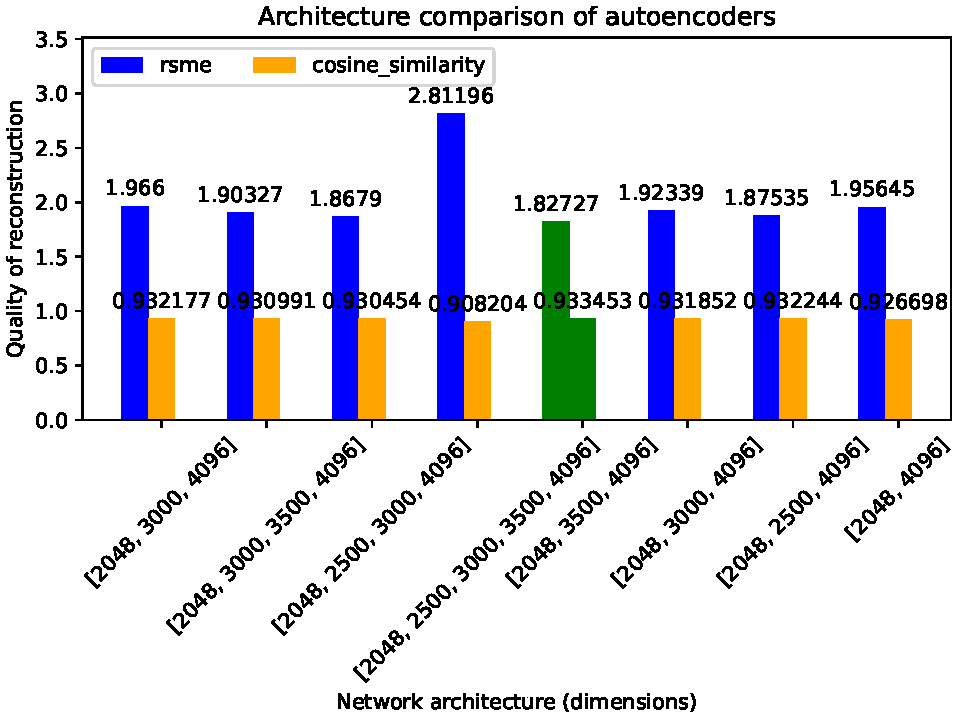
\includegraphics[width=0.7\textwidth]{images/embeddings/autoencoder/ae_score_plot.pdf}
    \caption[Different \ac{ae} architectures and their reconstruction error]{The effect of different \ac{ae} architectures on the reconstruction error.
    The error is measured in terms of \ac{rsme} (blue bars) and cosine similarity (yellow bars) between the original and the reconstructed image.
    The smallest \ac{rsme} and the biggest cosine similarity belong to the architecture best suitable to this task and are coloured green.
    }
    \label{fig:eval-ae-architecture}
\end{figure}